\documentclass[twoside]{book}

% Packages required by doxygen
\usepackage{fixltx2e}
\usepackage{calc}
\usepackage{doxygen}
\usepackage[export]{adjustbox} % also loads graphicx
\usepackage{graphicx}
\usepackage[utf8]{inputenc}
\usepackage{makeidx}
\usepackage{multicol}
\usepackage{multirow}
\PassOptionsToPackage{warn}{textcomp}
\usepackage{textcomp}
\usepackage[nointegrals]{wasysym}
\usepackage[table]{xcolor}

% Font selection
\usepackage[T1]{fontenc}
\usepackage[scaled=.90]{helvet}
\usepackage{courier}
\usepackage{amssymb}
\usepackage{sectsty}
\renewcommand{\familydefault}{\sfdefault}
\allsectionsfont{%
  \fontseries{bc}\selectfont%
  \color{darkgray}%
}
\renewcommand{\DoxyLabelFont}{%
  \fontseries{bc}\selectfont%
  \color{darkgray}%
}
\newcommand{\+}{\discretionary{\mbox{\scriptsize$\hookleftarrow$}}{}{}}

% Page & text layout
\usepackage{geometry}
\geometry{%
  a4paper,%
  top=2.5cm,%
  bottom=2.5cm,%
  left=2.5cm,%
  right=2.5cm%
}
\tolerance=750
\hfuzz=15pt
\hbadness=750
\setlength{\emergencystretch}{15pt}
\setlength{\parindent}{0cm}
\setlength{\parskip}{0.2cm}
\makeatletter
\renewcommand{\paragraph}{%
  \@startsection{paragraph}{4}{0ex}{-1.0ex}{1.0ex}{%
    \normalfont\normalsize\bfseries\SS@parafont%
  }%
}
\renewcommand{\subparagraph}{%
  \@startsection{subparagraph}{5}{0ex}{-1.0ex}{1.0ex}{%
    \normalfont\normalsize\bfseries\SS@subparafont%
  }%
}
\makeatother

% Headers & footers
\usepackage{fancyhdr}
\pagestyle{fancyplain}
\fancyhead[LE]{\fancyplain{}{\bfseries\thepage}}
\fancyhead[CE]{\fancyplain{}{}}
\fancyhead[RE]{\fancyplain{}{\bfseries\leftmark}}
\fancyhead[LO]{\fancyplain{}{\bfseries\rightmark}}
\fancyhead[CO]{\fancyplain{}{}}
\fancyhead[RO]{\fancyplain{}{\bfseries\thepage}}
\fancyfoot[LE]{\fancyplain{}{}}
\fancyfoot[CE]{\fancyplain{}{}}
\fancyfoot[RE]{\fancyplain{}{\bfseries\scriptsize Generated on Thu Jan 12 2017 07\+:17\+:29 for My Project by Doxygen }}
\fancyfoot[LO]{\fancyplain{}{\bfseries\scriptsize Generated on Thu Jan 12 2017 07\+:17\+:29 for My Project by Doxygen }}
\fancyfoot[CO]{\fancyplain{}{}}
\fancyfoot[RO]{\fancyplain{}{}}
\renewcommand{\footrulewidth}{0.4pt}
\renewcommand{\chaptermark}[1]{%
  \markboth{#1}{}%
}
\renewcommand{\sectionmark}[1]{%
  \markright{\thesection\ #1}%
}

% Indices & bibliography
\usepackage{natbib}
\usepackage[titles]{tocloft}
\setcounter{tocdepth}{3}
\setcounter{secnumdepth}{5}
\makeindex

% Hyperlinks (required, but should be loaded last)
\usepackage{ifpdf}
\ifpdf
  \usepackage[pdftex,pagebackref=true]{hyperref}
\else
  \usepackage[ps2pdf,pagebackref=true]{hyperref}
\fi
\hypersetup{%
  colorlinks=true,%
  linkcolor=blue,%
  citecolor=blue,%
  unicode%
}

% Custom commands
\newcommand{\clearemptydoublepage}{%
  \newpage{\pagestyle{empty}\cleardoublepage}%
}


%===== C O N T E N T S =====

\begin{document}

% Titlepage & ToC
\hypersetup{pageanchor=false,
             bookmarks=true,
             bookmarksnumbered=true,
             pdfencoding=unicode
            }
\pagenumbering{roman}
\begin{titlepage}
\vspace*{7cm}
\begin{center}%
{\Large My Project }\\
\vspace*{1cm}
{\large Generated by Doxygen 1.8.10}\\
\vspace*{0.5cm}
{\small Thu Jan 12 2017 07:17:29}\\
\end{center}
\end{titlepage}
\clearemptydoublepage
\tableofcontents
\clearemptydoublepage
\pagenumbering{arabic}
\hypersetup{pageanchor=true}

%--- Begin generated contents ---
\chapter{Namespace Index}
\section{Namespace List}
Here is a list of all namespaces with brief descriptions\+:\begin{DoxyCompactList}
\item\contentsline{section}{\hyperlink{namespace_util}{Util} }{\pageref{namespace_util}}{}
\end{DoxyCompactList}

\chapter{Hierarchical Index}
\section{Class Hierarchy}
This inheritance list is sorted roughly, but not completely, alphabetically\+:\begin{DoxyCompactList}
\item \contentsline{section}{Curl\+Cpp\+:\+:Curl\+Cpp}{\pageref{class_curl_cpp_1_1_curl_cpp}}{}
\item exception\begin{DoxyCompactList}
\item \contentsline{section}{Curl\+Cpp\+:\+:Curl\+Cpp\+Exception}{\pageref{class_curl_cpp_1_1_curl_cpp_exception}}{}
\end{DoxyCompactList}
\item \contentsline{section}{Mongo\+Client}{\pageref{class_mongo_client}}{}
\item Q\+Widget\begin{DoxyCompactList}
\item \contentsline{section}{Mainwindow}{\pageref{class_mainwindow}}{}
\end{DoxyCompactList}
\end{DoxyCompactList}

\chapter{Class Index}
\section{Class List}
Here are the classes, structs, unions and interfaces with brief descriptions\+:\begin{DoxyCompactList}
\item\contentsline{section}{\hyperlink{class_curl_cpp_1_1_curl_cpp}{Curl\+Cpp\+::\+Curl\+Cpp} }{\pageref{class_curl_cpp_1_1_curl_cpp}}{}
\item\contentsline{section}{\hyperlink{class_curl_cpp_1_1_curl_cpp_exception}{Curl\+Cpp\+::\+Curl\+Cpp\+Exception} }{\pageref{class_curl_cpp_1_1_curl_cpp_exception}}{}
\item\contentsline{section}{\hyperlink{class_mainwindow}{Mainwindow} }{\pageref{class_mainwindow}}{}
\item\contentsline{section}{\hyperlink{class_mongo_client}{Mongo\+Client} \\*Mongo client wrapper Mongo client wrapper helps creating a client for a mongo db }{\pageref{class_mongo_client}}{}
\end{DoxyCompactList}

\chapter{File Index}
\section{File List}
Here is a list of all files with brief descriptions\+:\begin{DoxyCompactList}
\item\contentsline{section}{/\+Users/mehdikhemir/\+Documents/\+Codes/\+Cpp/my\+App/src/\hyperlink{main_8cpp}{main.\+cpp} }{\pageref{main_8cpp}}{}
\item\contentsline{section}{/\+Users/mehdikhemir/\+Documents/\+Codes/\+Cpp/my\+App/src/\+Curl\+Cpp/\hyperlink{_curl_cpp_8cpp}{Curl\+Cpp.\+cpp} }{\pageref{_curl_cpp_8cpp}}{}
\item\contentsline{section}{/\+Users/mehdikhemir/\+Documents/\+Codes/\+Cpp/my\+App/src/\+Curl\+Cpp/\hyperlink{_curl_cpp_8hpp}{Curl\+Cpp.\+hpp} }{\pageref{_curl_cpp_8hpp}}{}
\item\contentsline{section}{/\+Users/mehdikhemir/\+Documents/\+Codes/\+Cpp/my\+App/src/\+Curl\+Cpp/\hyperlink{_curl_cpp_exception_8cpp}{Curl\+Cpp\+Exception.\+cpp} }{\pageref{_curl_cpp_exception_8cpp}}{}
\item\contentsline{section}{/\+Users/mehdikhemir/\+Documents/\+Codes/\+Cpp/my\+App/src/\+Curl\+Cpp/\hyperlink{_curl_cpp_exception_8hpp}{Curl\+Cpp\+Exception.\+hpp} }{\pageref{_curl_cpp_exception_8hpp}}{}
\item\contentsline{section}{/\+Users/mehdikhemir/\+Documents/\+Codes/\+Cpp/my\+App/src/\+Mainwindow/\hyperlink{_mainwindow_8cpp}{Mainwindow.\+cpp} }{\pageref{_mainwindow_8cpp}}{}
\item\contentsline{section}{/\+Users/mehdikhemir/\+Documents/\+Codes/\+Cpp/my\+App/src/\+Mainwindow/\hyperlink{_mainwindow_8hpp}{Mainwindow.\+hpp} }{\pageref{_mainwindow_8hpp}}{}
\item\contentsline{section}{/\+Users/mehdikhemir/\+Documents/\+Codes/\+Cpp/my\+App/src/\+Mongo\+Client/\hyperlink{_mongo_client_8cpp}{Mongo\+Client.\+cpp} }{\pageref{_mongo_client_8cpp}}{}
\item\contentsline{section}{/\+Users/mehdikhemir/\+Documents/\+Codes/\+Cpp/my\+App/src/\+Mongo\+Client/\hyperlink{_mongo_client_8hpp}{Mongo\+Client.\+hpp} }{\pageref{_mongo_client_8hpp}}{}
\item\contentsline{section}{/\+Users/mehdikhemir/\+Documents/\+Codes/\+Cpp/my\+App/src/\+Util/\hyperlink{_util_8cpp}{Util.\+cpp} }{\pageref{_util_8cpp}}{}
\item\contentsline{section}{/\+Users/mehdikhemir/\+Documents/\+Codes/\+Cpp/my\+App/src/\+Util/\hyperlink{_util_8hpp}{Util.\+hpp} }{\pageref{_util_8hpp}}{}
\end{DoxyCompactList}

\chapter{Namespace Documentation}
\hypertarget{namespace_curl_cpp}{}\section{Curl\+Cpp Namespace Reference}
\label{namespace_curl_cpp}\index{Curl\+Cpp@{Curl\+Cpp}}
\subsection*{Classes}
\begin{DoxyCompactItemize}
\item 
class \hyperlink{class_curl_cpp_1_1_curl_cpp}{Curl\+Cpp}
\item 
class \hyperlink{class_curl_cpp_1_1_curl_cpp_exception}{Curl\+Cpp\+Exception}
\end{DoxyCompactItemize}

\hypertarget{namespace_util}{}\section{Util Namespace Reference}
\label{namespace_util}\index{Util@{Util}}
\subsection*{Functions}
\begin{DoxyCompactItemize}
\item 
std\+::vector$<$ std\+::string $>$ \hyperlink{namespace_util_a86f16dfe1bb012de7a48f5e19ffa9279}{parse\+String} (std\+::string input, char separator)
\end{DoxyCompactItemize}


\subsection{Function Documentation}
\hypertarget{namespace_util_a86f16dfe1bb012de7a48f5e19ffa9279}{}\index{Util@{Util}!parse\+String@{parse\+String}}
\index{parse\+String@{parse\+String}!Util@{Util}}
\subsubsection[{parse\+String(std\+::string input, char separator)}]{\setlength{\rightskip}{0pt plus 5cm}std\+::vector$<$ std\+::string $>$ Util\+::parse\+String (
\begin{DoxyParamCaption}
\item[{std\+::string}]{input, }
\item[{char}]{separator}
\end{DoxyParamCaption}
)}\label{namespace_util_a86f16dfe1bb012de7a48f5e19ffa9279}

\chapter{Class Documentation}
\hypertarget{class_curl_cpp_1_1_curl_cpp}{}\section{Curl\+Cpp\+:\+:Curl\+Cpp Class Reference}
\label{class_curl_cpp_1_1_curl_cpp}\index{Curl\+Cpp\+::\+Curl\+Cpp@{Curl\+Cpp\+::\+Curl\+Cpp}}


{\ttfamily \#include $<$Curl\+Cpp.\+hpp$>$}

\subsection*{Public Member Functions}
\begin{DoxyCompactItemize}
\item 
\hyperlink{class_curl_cpp_1_1_curl_cpp_a00e67f746846377c451d915e83c564bf}{Curl\+Cpp} ()
\item 
\hyperlink{class_curl_cpp_1_1_curl_cpp_aeb659c8fb3d12f4a6e363fca418785dc}{$\sim$\+Curl\+Cpp} ()
\item 
void \hyperlink{class_curl_cpp_1_1_curl_cpp_afe16ac5d787c709cc04ebaf57afbfaa2}{append\+Headers} (std\+::string new\+Header)
\item 
curl\+\_\+slist $\ast$ \hyperlink{class_curl_cpp_1_1_curl_cpp_a9fad186212d2258e1f26e2d4b9dad498}{get\+Headers} ()
\item 
std\+::vector$<$ std\+::string $>$ \hyperlink{class_curl_cpp_1_1_curl_cpp_a0603b5b5a02bb86d2a2cb9e7e2385561}{get\+Vec\+Str\+Headers} ()
\item 
void \hyperlink{class_curl_cpp_1_1_curl_cpp_ade54efe4f6b4427b4df32bf84957b307}{add\+Url} (std\+::string url\+Port)
\item 
std\+::vector$<$ std\+::string $>$ \hyperlink{class_curl_cpp_1_1_curl_cpp_abc13a0fc97bdada59643ffad51b73387}{from\+List\+To\+Vector} ()
\end{DoxyCompactItemize}
\subsection*{Private Attributes}
\begin{DoxyCompactItemize}
\item 
curl\+\_\+slist $\ast$ \hyperlink{class_curl_cpp_1_1_curl_cpp_ada5ea161e25d1f657d0646067d843afc}{headers}
\item 
C\+U\+R\+Lcode \hyperlink{class_curl_cpp_1_1_curl_cpp_affd7aa2823468685baf06ba790f50dc4}{\+\_\+curl\+Init\+Code}
\item 
curl\+\_\+slist $\ast$ \hyperlink{class_curl_cpp_1_1_curl_cpp_a683cf293e1868db0ca6753ad8a5cd7d2}{\+\_\+headers}
\item 
C\+U\+R\+L $\ast$ \hyperlink{class_curl_cpp_1_1_curl_cpp_a51adae9da8e6effe1ff6cddce45f026e}{\+\_\+curl\+Handler}
\item 
std\+::vector$<$ std\+::string $>$ \hyperlink{class_curl_cpp_1_1_curl_cpp_acd6960ca4b1abe99aa00bca6a24dcace}{\+\_\+vec\+Str\+Headers}
\end{DoxyCompactItemize}


\subsection{Constructor \& Destructor Documentation}
\hypertarget{class_curl_cpp_1_1_curl_cpp_a00e67f746846377c451d915e83c564bf}{}\index{Curl\+Cpp\+::\+Curl\+Cpp@{Curl\+Cpp\+::\+Curl\+Cpp}!Curl\+Cpp@{Curl\+Cpp}}
\index{Curl\+Cpp@{Curl\+Cpp}!Curl\+Cpp\+::\+Curl\+Cpp@{Curl\+Cpp\+::\+Curl\+Cpp}}
\subsubsection[{Curl\+Cpp()}]{\setlength{\rightskip}{0pt plus 5cm}Curl\+Cpp\+::\+Curl\+Cpp\+::\+Curl\+Cpp (
\begin{DoxyParamCaption}
{}
\end{DoxyParamCaption}
)}\label{class_curl_cpp_1_1_curl_cpp_a00e67f746846377c451d915e83c564bf}
\hypertarget{class_curl_cpp_1_1_curl_cpp_aeb659c8fb3d12f4a6e363fca418785dc}{}\index{Curl\+Cpp\+::\+Curl\+Cpp@{Curl\+Cpp\+::\+Curl\+Cpp}!````~Curl\+Cpp@{$\sim$\+Curl\+Cpp}}
\index{````~Curl\+Cpp@{$\sim$\+Curl\+Cpp}!Curl\+Cpp\+::\+Curl\+Cpp@{Curl\+Cpp\+::\+Curl\+Cpp}}
\subsubsection[{$\sim$\+Curl\+Cpp()}]{\setlength{\rightskip}{0pt plus 5cm}Curl\+Cpp\+::\+Curl\+Cpp\+::$\sim$\+Curl\+Cpp (
\begin{DoxyParamCaption}
{}
\end{DoxyParamCaption}
)}\label{class_curl_cpp_1_1_curl_cpp_aeb659c8fb3d12f4a6e363fca418785dc}


\subsection{Member Function Documentation}
\hypertarget{class_curl_cpp_1_1_curl_cpp_ade54efe4f6b4427b4df32bf84957b307}{}\index{Curl\+Cpp\+::\+Curl\+Cpp@{Curl\+Cpp\+::\+Curl\+Cpp}!add\+Url@{add\+Url}}
\index{add\+Url@{add\+Url}!Curl\+Cpp\+::\+Curl\+Cpp@{Curl\+Cpp\+::\+Curl\+Cpp}}
\subsubsection[{add\+Url(std\+::string url\+Port)}]{\setlength{\rightskip}{0pt plus 5cm}void Curl\+Cpp\+::\+Curl\+Cpp\+::add\+Url (
\begin{DoxyParamCaption}
\item[{std\+::string}]{url\+Port}
\end{DoxyParamCaption}
)}\label{class_curl_cpp_1_1_curl_cpp_ade54efe4f6b4427b4df32bf84957b307}
\hypertarget{class_curl_cpp_1_1_curl_cpp_afe16ac5d787c709cc04ebaf57afbfaa2}{}\index{Curl\+Cpp\+::\+Curl\+Cpp@{Curl\+Cpp\+::\+Curl\+Cpp}!append\+Headers@{append\+Headers}}
\index{append\+Headers@{append\+Headers}!Curl\+Cpp\+::\+Curl\+Cpp@{Curl\+Cpp\+::\+Curl\+Cpp}}
\subsubsection[{append\+Headers(std\+::string new\+Header)}]{\setlength{\rightskip}{0pt plus 5cm}void Curl\+Cpp\+::\+Curl\+Cpp\+::append\+Headers (
\begin{DoxyParamCaption}
\item[{std\+::string}]{new\+Header}
\end{DoxyParamCaption}
)}\label{class_curl_cpp_1_1_curl_cpp_afe16ac5d787c709cc04ebaf57afbfaa2}
\hypertarget{class_curl_cpp_1_1_curl_cpp_abc13a0fc97bdada59643ffad51b73387}{}\index{Curl\+Cpp\+::\+Curl\+Cpp@{Curl\+Cpp\+::\+Curl\+Cpp}!from\+List\+To\+Vector@{from\+List\+To\+Vector}}
\index{from\+List\+To\+Vector@{from\+List\+To\+Vector}!Curl\+Cpp\+::\+Curl\+Cpp@{Curl\+Cpp\+::\+Curl\+Cpp}}
\subsubsection[{from\+List\+To\+Vector()}]{\setlength{\rightskip}{0pt plus 5cm}std\+::vector$<$ std\+::string $>$ Curl\+Cpp\+::\+Curl\+Cpp\+::from\+List\+To\+Vector (
\begin{DoxyParamCaption}
{}
\end{DoxyParamCaption}
)}\label{class_curl_cpp_1_1_curl_cpp_abc13a0fc97bdada59643ffad51b73387}
\hypertarget{class_curl_cpp_1_1_curl_cpp_a9fad186212d2258e1f26e2d4b9dad498}{}\index{Curl\+Cpp\+::\+Curl\+Cpp@{Curl\+Cpp\+::\+Curl\+Cpp}!get\+Headers@{get\+Headers}}
\index{get\+Headers@{get\+Headers}!Curl\+Cpp\+::\+Curl\+Cpp@{Curl\+Cpp\+::\+Curl\+Cpp}}
\subsubsection[{get\+Headers()}]{\setlength{\rightskip}{0pt plus 5cm}curl\+\_\+slist $\ast$ Curl\+Cpp\+::\+Curl\+Cpp\+::get\+Headers (
\begin{DoxyParamCaption}
{}
\end{DoxyParamCaption}
)}\label{class_curl_cpp_1_1_curl_cpp_a9fad186212d2258e1f26e2d4b9dad498}
\hypertarget{class_curl_cpp_1_1_curl_cpp_a0603b5b5a02bb86d2a2cb9e7e2385561}{}\index{Curl\+Cpp\+::\+Curl\+Cpp@{Curl\+Cpp\+::\+Curl\+Cpp}!get\+Vec\+Str\+Headers@{get\+Vec\+Str\+Headers}}
\index{get\+Vec\+Str\+Headers@{get\+Vec\+Str\+Headers}!Curl\+Cpp\+::\+Curl\+Cpp@{Curl\+Cpp\+::\+Curl\+Cpp}}
\subsubsection[{get\+Vec\+Str\+Headers()}]{\setlength{\rightskip}{0pt plus 5cm}std\+::vector$<$ std\+::string $>$ Curl\+Cpp\+::\+Curl\+Cpp\+::get\+Vec\+Str\+Headers (
\begin{DoxyParamCaption}
{}
\end{DoxyParamCaption}
)}\label{class_curl_cpp_1_1_curl_cpp_a0603b5b5a02bb86d2a2cb9e7e2385561}


\subsection{Member Data Documentation}
\hypertarget{class_curl_cpp_1_1_curl_cpp_a51adae9da8e6effe1ff6cddce45f026e}{}\index{Curl\+Cpp\+::\+Curl\+Cpp@{Curl\+Cpp\+::\+Curl\+Cpp}!\+\_\+curl\+Handler@{\+\_\+curl\+Handler}}
\index{\+\_\+curl\+Handler@{\+\_\+curl\+Handler}!Curl\+Cpp\+::\+Curl\+Cpp@{Curl\+Cpp\+::\+Curl\+Cpp}}
\subsubsection[{\+\_\+curl\+Handler}]{\setlength{\rightskip}{0pt plus 5cm}C\+U\+R\+L$\ast$ Curl\+Cpp\+::\+Curl\+Cpp\+::\+\_\+curl\+Handler\hspace{0.3cm}{\ttfamily [private]}}\label{class_curl_cpp_1_1_curl_cpp_a51adae9da8e6effe1ff6cddce45f026e}
\hypertarget{class_curl_cpp_1_1_curl_cpp_affd7aa2823468685baf06ba790f50dc4}{}\index{Curl\+Cpp\+::\+Curl\+Cpp@{Curl\+Cpp\+::\+Curl\+Cpp}!\+\_\+curl\+Init\+Code@{\+\_\+curl\+Init\+Code}}
\index{\+\_\+curl\+Init\+Code@{\+\_\+curl\+Init\+Code}!Curl\+Cpp\+::\+Curl\+Cpp@{Curl\+Cpp\+::\+Curl\+Cpp}}
\subsubsection[{\+\_\+curl\+Init\+Code}]{\setlength{\rightskip}{0pt plus 5cm}C\+U\+R\+Lcode Curl\+Cpp\+::\+Curl\+Cpp\+::\+\_\+curl\+Init\+Code\hspace{0.3cm}{\ttfamily [private]}}\label{class_curl_cpp_1_1_curl_cpp_affd7aa2823468685baf06ba790f50dc4}
\hypertarget{class_curl_cpp_1_1_curl_cpp_a683cf293e1868db0ca6753ad8a5cd7d2}{}\index{Curl\+Cpp\+::\+Curl\+Cpp@{Curl\+Cpp\+::\+Curl\+Cpp}!\+\_\+headers@{\+\_\+headers}}
\index{\+\_\+headers@{\+\_\+headers}!Curl\+Cpp\+::\+Curl\+Cpp@{Curl\+Cpp\+::\+Curl\+Cpp}}
\subsubsection[{\+\_\+headers}]{\setlength{\rightskip}{0pt plus 5cm}curl\+\_\+slist$\ast$ Curl\+Cpp\+::\+Curl\+Cpp\+::\+\_\+headers\hspace{0.3cm}{\ttfamily [private]}}\label{class_curl_cpp_1_1_curl_cpp_a683cf293e1868db0ca6753ad8a5cd7d2}
\hypertarget{class_curl_cpp_1_1_curl_cpp_acd6960ca4b1abe99aa00bca6a24dcace}{}\index{Curl\+Cpp\+::\+Curl\+Cpp@{Curl\+Cpp\+::\+Curl\+Cpp}!\+\_\+vec\+Str\+Headers@{\+\_\+vec\+Str\+Headers}}
\index{\+\_\+vec\+Str\+Headers@{\+\_\+vec\+Str\+Headers}!Curl\+Cpp\+::\+Curl\+Cpp@{Curl\+Cpp\+::\+Curl\+Cpp}}
\subsubsection[{\+\_\+vec\+Str\+Headers}]{\setlength{\rightskip}{0pt plus 5cm}std\+::vector$<$std\+::string$>$ Curl\+Cpp\+::\+Curl\+Cpp\+::\+\_\+vec\+Str\+Headers\hspace{0.3cm}{\ttfamily [private]}}\label{class_curl_cpp_1_1_curl_cpp_acd6960ca4b1abe99aa00bca6a24dcace}
\hypertarget{class_curl_cpp_1_1_curl_cpp_ada5ea161e25d1f657d0646067d843afc}{}\index{Curl\+Cpp\+::\+Curl\+Cpp@{Curl\+Cpp\+::\+Curl\+Cpp}!headers@{headers}}
\index{headers@{headers}!Curl\+Cpp\+::\+Curl\+Cpp@{Curl\+Cpp\+::\+Curl\+Cpp}}
\subsubsection[{headers}]{\setlength{\rightskip}{0pt plus 5cm}curl\+\_\+slist$\ast$ Curl\+Cpp\+::\+Curl\+Cpp\+::headers\hspace{0.3cm}{\ttfamily [private]}}\label{class_curl_cpp_1_1_curl_cpp_ada5ea161e25d1f657d0646067d843afc}


The documentation for this class was generated from the following files\+:\begin{DoxyCompactItemize}
\item 
/\+Users/mehdikhemir/\+Documents/\+Codes/\+Cpp/my\+App/src/\+Curl\+Cpp/\hyperlink{_curl_cpp_8hpp}{Curl\+Cpp.\+hpp}\item 
/\+Users/mehdikhemir/\+Documents/\+Codes/\+Cpp/my\+App/src/\+Curl\+Cpp/\hyperlink{_curl_cpp_8cpp}{Curl\+Cpp.\+cpp}\end{DoxyCompactItemize}

\hypertarget{class_curl_cpp_1_1_curl_cpp_exception}{}\section{Curl\+Cpp\+:\+:Curl\+Cpp\+Exception Class Reference}
\label{class_curl_cpp_1_1_curl_cpp_exception}\index{Curl\+Cpp\+::\+Curl\+Cpp\+Exception@{Curl\+Cpp\+::\+Curl\+Cpp\+Exception}}


{\ttfamily \#include $<$Curl\+Cpp\+Exception.\+hpp$>$}

Inheritance diagram for Curl\+Cpp\+:\+:Curl\+Cpp\+Exception\+:\begin{figure}[H]
\begin{center}
\leavevmode
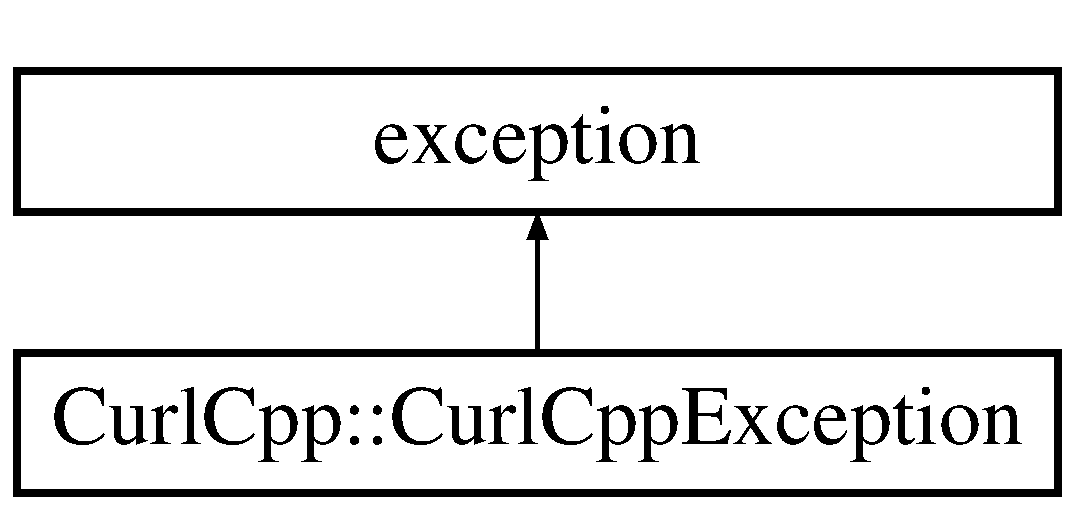
\includegraphics[height=2.000000cm]{class_curl_cpp_1_1_curl_cpp_exception}
\end{center}
\end{figure}
\subsection*{Public Member Functions}
\begin{DoxyCompactItemize}
\item 
\hyperlink{class_curl_cpp_1_1_curl_cpp_exception_a0511de152c15c19174051a5b9045becf}{Curl\+Cpp\+Exception} (std\+::string error\+Message)
\item 
virtual const char $\ast$ \hyperlink{class_curl_cpp_1_1_curl_cpp_exception_a24b4be0db92a900b2779752d178f80c8}{what} () const   throw ()
\end{DoxyCompactItemize}
\subsection*{Private Attributes}
\begin{DoxyCompactItemize}
\item 
std\+::string \hyperlink{class_curl_cpp_1_1_curl_cpp_exception_a09d95a9e9d9f9cf400fb51784d22d0d2}{\+\_\+error\+Message}
\end{DoxyCompactItemize}


\subsection{Constructor \& Destructor Documentation}
\hypertarget{class_curl_cpp_1_1_curl_cpp_exception_a0511de152c15c19174051a5b9045becf}{}\index{Curl\+Cpp\+::\+Curl\+Cpp\+Exception@{Curl\+Cpp\+::\+Curl\+Cpp\+Exception}!Curl\+Cpp\+Exception@{Curl\+Cpp\+Exception}}
\index{Curl\+Cpp\+Exception@{Curl\+Cpp\+Exception}!Curl\+Cpp\+::\+Curl\+Cpp\+Exception@{Curl\+Cpp\+::\+Curl\+Cpp\+Exception}}
\subsubsection[{Curl\+Cpp\+Exception(std\+::string error\+Message)}]{\setlength{\rightskip}{0pt plus 5cm}Curl\+Cpp\+::\+Curl\+Cpp\+Exception\+::\+Curl\+Cpp\+Exception (
\begin{DoxyParamCaption}
\item[{std\+::string}]{error\+Message}
\end{DoxyParamCaption}
)}\label{class_curl_cpp_1_1_curl_cpp_exception_a0511de152c15c19174051a5b9045becf}


\subsection{Member Function Documentation}
\hypertarget{class_curl_cpp_1_1_curl_cpp_exception_a24b4be0db92a900b2779752d178f80c8}{}\index{Curl\+Cpp\+::\+Curl\+Cpp\+Exception@{Curl\+Cpp\+::\+Curl\+Cpp\+Exception}!what@{what}}
\index{what@{what}!Curl\+Cpp\+::\+Curl\+Cpp\+Exception@{Curl\+Cpp\+::\+Curl\+Cpp\+Exception}}
\subsubsection[{what() const }]{\setlength{\rightskip}{0pt plus 5cm}const char $\ast$ Curl\+Cpp\+::\+Curl\+Cpp\+Exception\+::what (
\begin{DoxyParamCaption}
{}
\end{DoxyParamCaption}
) const throw  ) \hspace{0.3cm}{\ttfamily [virtual]}}\label{class_curl_cpp_1_1_curl_cpp_exception_a24b4be0db92a900b2779752d178f80c8}


\subsection{Member Data Documentation}
\hypertarget{class_curl_cpp_1_1_curl_cpp_exception_a09d95a9e9d9f9cf400fb51784d22d0d2}{}\index{Curl\+Cpp\+::\+Curl\+Cpp\+Exception@{Curl\+Cpp\+::\+Curl\+Cpp\+Exception}!\+\_\+error\+Message@{\+\_\+error\+Message}}
\index{\+\_\+error\+Message@{\+\_\+error\+Message}!Curl\+Cpp\+::\+Curl\+Cpp\+Exception@{Curl\+Cpp\+::\+Curl\+Cpp\+Exception}}
\subsubsection[{\+\_\+error\+Message}]{\setlength{\rightskip}{0pt plus 5cm}std\+::string Curl\+Cpp\+::\+Curl\+Cpp\+Exception\+::\+\_\+error\+Message\hspace{0.3cm}{\ttfamily [private]}}\label{class_curl_cpp_1_1_curl_cpp_exception_a09d95a9e9d9f9cf400fb51784d22d0d2}


The documentation for this class was generated from the following files\+:\begin{DoxyCompactItemize}
\item 
/\+Users/mehdikhemir/\+Documents/\+Codes/\+Cpp/my\+App/src/\+Curl\+Cpp/\hyperlink{_curl_cpp_exception_8hpp}{Curl\+Cpp\+Exception.\+hpp}\item 
/\+Users/mehdikhemir/\+Documents/\+Codes/\+Cpp/my\+App/src/\+Curl\+Cpp/\hyperlink{_curl_cpp_exception_8cpp}{Curl\+Cpp\+Exception.\+cpp}\end{DoxyCompactItemize}

\hypertarget{class_mainwindow}{}\section{Mainwindow Class Reference}
\label{class_mainwindow}\index{Mainwindow@{Mainwindow}}


{\ttfamily \#include $<$Mainwindow.\+hpp$>$}

Inheritance diagram for Mainwindow\+:\begin{figure}[H]
\begin{center}
\leavevmode
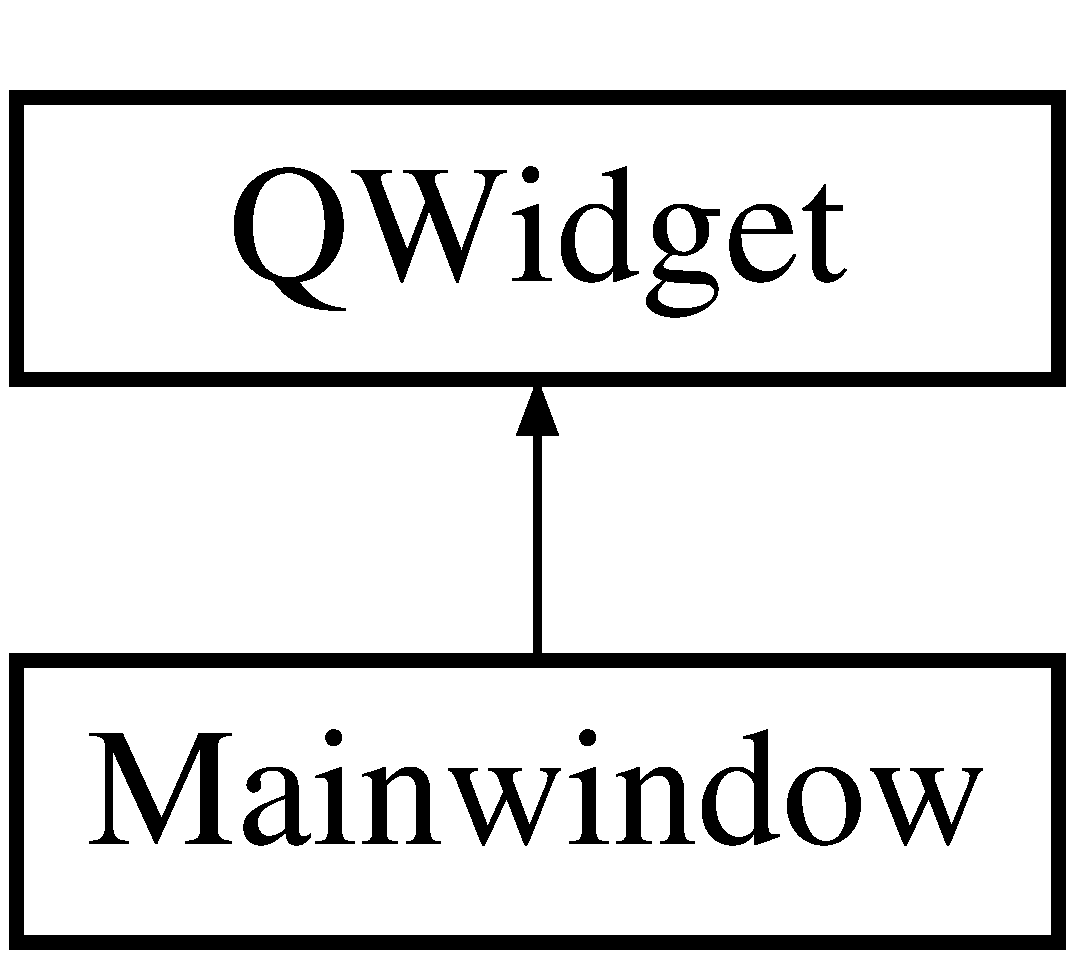
\includegraphics[height=2.000000cm]{class_mainwindow}
\end{center}
\end{figure}
\subsection*{Public Slots}
\begin{DoxyCompactItemize}
\item 
void \hyperlink{class_mainwindow_ab3176d338d0345c6e777dab74b742a33}{change\+Width} (int width)
\end{DoxyCompactItemize}
\subsection*{Static Public Member Functions}
\begin{DoxyCompactItemize}
\item 
static \hyperlink{class_mainwindow}{Mainwindow} $\ast$ \hyperlink{class_mainwindow_aedafe213d761a416bae8ccaffa6410b0}{instance} ()
\end{DoxyCompactItemize}
\subsection*{Private Member Functions}
\begin{DoxyCompactItemize}
\item 
\hyperlink{class_mainwindow_a9ca049b84f17c87a57b53e418b1c40e3}{Mainwindow} ()
\end{DoxyCompactItemize}
\subsection*{Private Attributes}
\begin{DoxyCompactItemize}
\item 
Q\+L\+C\+D\+Number $\ast$ \hyperlink{class_mainwindow_abd18cf97d805d3ea3c9d00937078b4f4}{m\+\_\+lcd}
\item 
Q\+Slider $\ast$ \hyperlink{class_mainwindow_af706665f6371f479b89bc5cd722191df}{m\+\_\+slider}
\item 
Q\+Push\+Button $\ast$ \hyperlink{class_mainwindow_a64a43df893109c11db9482ba2d7646dc}{m\+\_\+pushbutton}
\end{DoxyCompactItemize}
\subsection*{Static Private Attributes}
\begin{DoxyCompactItemize}
\item 
static \hyperlink{class_mainwindow}{Mainwindow} $\ast$ \hyperlink{class_mainwindow_a47858f9db0a0c89d7df36cb56925118d}{s\+\_\+instance} = N\+U\+L\+L
\end{DoxyCompactItemize}


\subsection{Constructor \& Destructor Documentation}
\hypertarget{class_mainwindow_a9ca049b84f17c87a57b53e418b1c40e3}{}\index{Mainwindow@{Mainwindow}!Mainwindow@{Mainwindow}}
\index{Mainwindow@{Mainwindow}!Mainwindow@{Mainwindow}}
\subsubsection[{Mainwindow()}]{\setlength{\rightskip}{0pt plus 5cm}Mainwindow\+::\+Mainwindow (
\begin{DoxyParamCaption}
{}
\end{DoxyParamCaption}
)\hspace{0.3cm}{\ttfamily [private]}}\label{class_mainwindow_a9ca049b84f17c87a57b53e418b1c40e3}


\subsection{Member Function Documentation}
\hypertarget{class_mainwindow_ab3176d338d0345c6e777dab74b742a33}{}\index{Mainwindow@{Mainwindow}!change\+Width@{change\+Width}}
\index{change\+Width@{change\+Width}!Mainwindow@{Mainwindow}}
\subsubsection[{change\+Width}]{\setlength{\rightskip}{0pt plus 5cm}void Mainwindow\+::change\+Width (
\begin{DoxyParamCaption}
\item[{int}]{width}
\end{DoxyParamCaption}
)\hspace{0.3cm}{\ttfamily [slot]}}\label{class_mainwindow_ab3176d338d0345c6e777dab74b742a33}
\hypertarget{class_mainwindow_aedafe213d761a416bae8ccaffa6410b0}{}\index{Mainwindow@{Mainwindow}!instance@{instance}}
\index{instance@{instance}!Mainwindow@{Mainwindow}}
\subsubsection[{instance()}]{\setlength{\rightskip}{0pt plus 5cm}{\bf Mainwindow} $\ast$ Mainwindow\+::instance (
\begin{DoxyParamCaption}
{}
\end{DoxyParamCaption}
)\hspace{0.3cm}{\ttfamily [static]}}\label{class_mainwindow_aedafe213d761a416bae8ccaffa6410b0}


\subsection{Member Data Documentation}
\hypertarget{class_mainwindow_abd18cf97d805d3ea3c9d00937078b4f4}{}\index{Mainwindow@{Mainwindow}!m\+\_\+lcd@{m\+\_\+lcd}}
\index{m\+\_\+lcd@{m\+\_\+lcd}!Mainwindow@{Mainwindow}}
\subsubsection[{m\+\_\+lcd}]{\setlength{\rightskip}{0pt plus 5cm}Q\+L\+C\+D\+Number$\ast$ Mainwindow\+::m\+\_\+lcd\hspace{0.3cm}{\ttfamily [private]}}\label{class_mainwindow_abd18cf97d805d3ea3c9d00937078b4f4}
\hypertarget{class_mainwindow_a64a43df893109c11db9482ba2d7646dc}{}\index{Mainwindow@{Mainwindow}!m\+\_\+pushbutton@{m\+\_\+pushbutton}}
\index{m\+\_\+pushbutton@{m\+\_\+pushbutton}!Mainwindow@{Mainwindow}}
\subsubsection[{m\+\_\+pushbutton}]{\setlength{\rightskip}{0pt plus 5cm}Q\+Push\+Button$\ast$ Mainwindow\+::m\+\_\+pushbutton\hspace{0.3cm}{\ttfamily [private]}}\label{class_mainwindow_a64a43df893109c11db9482ba2d7646dc}
\hypertarget{class_mainwindow_af706665f6371f479b89bc5cd722191df}{}\index{Mainwindow@{Mainwindow}!m\+\_\+slider@{m\+\_\+slider}}
\index{m\+\_\+slider@{m\+\_\+slider}!Mainwindow@{Mainwindow}}
\subsubsection[{m\+\_\+slider}]{\setlength{\rightskip}{0pt plus 5cm}Q\+Slider$\ast$ Mainwindow\+::m\+\_\+slider\hspace{0.3cm}{\ttfamily [private]}}\label{class_mainwindow_af706665f6371f479b89bc5cd722191df}
\hypertarget{class_mainwindow_a47858f9db0a0c89d7df36cb56925118d}{}\index{Mainwindow@{Mainwindow}!s\+\_\+instance@{s\+\_\+instance}}
\index{s\+\_\+instance@{s\+\_\+instance}!Mainwindow@{Mainwindow}}
\subsubsection[{s\+\_\+instance}]{\setlength{\rightskip}{0pt plus 5cm}{\bf Mainwindow} $\ast$ Mainwindow\+::s\+\_\+instance = N\+U\+L\+L\hspace{0.3cm}{\ttfamily [static]}, {\ttfamily [private]}}\label{class_mainwindow_a47858f9db0a0c89d7df36cb56925118d}


The documentation for this class was generated from the following files\+:\begin{DoxyCompactItemize}
\item 
/\+Users/mehdikhemir/\+Documents/\+Codes/\+Cpp/my\+App/src/\+Mainwindow/\hyperlink{_mainwindow_8hpp}{Mainwindow.\+hpp}\item 
/\+Users/mehdikhemir/\+Documents/\+Codes/\+Cpp/my\+App/src/\+Mainwindow/\hyperlink{_mainwindow_8cpp}{Mainwindow.\+cpp}\end{DoxyCompactItemize}

\hypertarget{class_mongo_client}{}\section{Mongo\+Client Class Reference}
\label{class_mongo_client}\index{Mongo\+Client@{Mongo\+Client}}


Mongo client wrapper Mongo client wrapper helps creating a client for a mongo db.  




{\ttfamily \#include $<$Mongo\+Client.\+hpp$>$}

\subsection*{Public Member Functions}
\begin{DoxyCompactItemize}
\item 
\hyperlink{class_mongo_client_a99c002f0875bafe7c72147aaed9086c0}{Mongo\+Client} (std\+::string uri, std\+::string db, std\+::string field\+\_\+name)
\item 
\hyperlink{class_mongo_client_aecb48220a940f8782861573a8b5d8692}{$\sim$\+Mongo\+Client} ()
\item 
std\+::vector$<$ std\+::string $>$ \hyperlink{class_mongo_client_af6a3081ec6f89b3f60eb4412807b172c}{get\+Collections} ()
\item 
std\+::vector$<$ std\+::string $>$ \hyperlink{class_mongo_client_ad5a0b939338a63f5dacc665056c8b330}{get\+Documents} (std\+::string in\+\_\+collection)
\end{DoxyCompactItemize}
\subsection*{Private Attributes}
\begin{DoxyCompactItemize}
\item 
mongocxx\+::uri $\ast$ \hyperlink{class_mongo_client_a0d5c8e1f21ef69de175ab07d7f074a22}{\+\_\+uri}
\item 
mongocxx\+::client $\ast$ \hyperlink{class_mongo_client_a5219540804d9229ab6a1da001c26a068}{\+\_\+client}
\item 
mongocxx\+::database $\ast$ \hyperlink{class_mongo_client_a1c48eda1d75c705898a8c04608f3f434}{\+\_\+db}
\item 
mongocxx\+::cursor $\ast$ \hyperlink{class_mongo_client_acee6b5e0d56b6ce9b99d363b7dc9d414}{\+\_\+cursor\+\_\+db}
\item 
mongocxx\+::collection \hyperlink{class_mongo_client_a68d5a96bba159d62203881ad6cc01912}{\+\_\+collection}
\item 
std\+::vector$<$ std\+::string $>$ \hyperlink{class_mongo_client_a0fe1acf7025dfc3ddaea718c5ab03746}{\+\_\+v\+\_\+collections}
\item 
std\+::string \hyperlink{class_mongo_client_ab3ded8c67af64c8b6b7a0a52da53a40f}{\+\_\+field\+\_\+name}
\end{DoxyCompactItemize}


\subsection{Detailed Description}
Mongo client wrapper Mongo client wrapper helps creating a client for a mongo db. 

\subsection{Constructor \& Destructor Documentation}
\hypertarget{class_mongo_client_a99c002f0875bafe7c72147aaed9086c0}{}\index{Mongo\+Client@{Mongo\+Client}!Mongo\+Client@{Mongo\+Client}}
\index{Mongo\+Client@{Mongo\+Client}!Mongo\+Client@{Mongo\+Client}}
\subsubsection[{Mongo\+Client(std\+::string uri, std\+::string db, std\+::string field\+\_\+name)}]{\setlength{\rightskip}{0pt plus 5cm}Mongo\+Client\+::\+Mongo\+Client (
\begin{DoxyParamCaption}
\item[{std\+::string}]{uri, }
\item[{std\+::string}]{db, }
\item[{std\+::string}]{field\+\_\+name}
\end{DoxyParamCaption}
)}\label{class_mongo_client_a99c002f0875bafe7c72147aaed9086c0}
Constructor 
\begin{DoxyParams}{Parameters}
{\em uri} & Address of the mongo db \\
\hline
{\em db} & Data\+Base you want to connect to \\
\hline
{\em field\+\_\+name} & Crappy stuff to put but necessary in order to extract the info of the documents \\
\hline
\end{DoxyParams}
\hypertarget{class_mongo_client_aecb48220a940f8782861573a8b5d8692}{}\index{Mongo\+Client@{Mongo\+Client}!````~Mongo\+Client@{$\sim$\+Mongo\+Client}}
\index{````~Mongo\+Client@{$\sim$\+Mongo\+Client}!Mongo\+Client@{Mongo\+Client}}
\subsubsection[{$\sim$\+Mongo\+Client()}]{\setlength{\rightskip}{0pt plus 5cm}Mongo\+Client\+::$\sim$\+Mongo\+Client (
\begin{DoxyParamCaption}
{}
\end{DoxyParamCaption}
)}\label{class_mongo_client_aecb48220a940f8782861573a8b5d8692}


\subsection{Member Function Documentation}
\hypertarget{class_mongo_client_af6a3081ec6f89b3f60eb4412807b172c}{}\index{Mongo\+Client@{Mongo\+Client}!get\+Collections@{get\+Collections}}
\index{get\+Collections@{get\+Collections}!Mongo\+Client@{Mongo\+Client}}
\subsubsection[{get\+Collections()}]{\setlength{\rightskip}{0pt plus 5cm}std\+::vector$<$ std\+::string $>$ Mongo\+Client\+::get\+Collections (
\begin{DoxyParamCaption}
{}
\end{DoxyParamCaption}
)}\label{class_mongo_client_af6a3081ec6f89b3f60eb4412807b172c}
Get all the collections of the selected database \hypertarget{class_mongo_client_ad5a0b939338a63f5dacc665056c8b330}{}\index{Mongo\+Client@{Mongo\+Client}!get\+Documents@{get\+Documents}}
\index{get\+Documents@{get\+Documents}!Mongo\+Client@{Mongo\+Client}}
\subsubsection[{get\+Documents(std\+::string in\+\_\+collection)}]{\setlength{\rightskip}{0pt plus 5cm}std\+::vector$<$ std\+::string $>$ Mongo\+Client\+::get\+Documents (
\begin{DoxyParamCaption}
\item[{std\+::string}]{in\+\_\+collection}
\end{DoxyParamCaption}
)}\label{class_mongo_client_ad5a0b939338a63f5dacc665056c8b330}
Get all documents from the collection selected 

\subsection{Member Data Documentation}
\hypertarget{class_mongo_client_a5219540804d9229ab6a1da001c26a068}{}\index{Mongo\+Client@{Mongo\+Client}!\+\_\+client@{\+\_\+client}}
\index{\+\_\+client@{\+\_\+client}!Mongo\+Client@{Mongo\+Client}}
\subsubsection[{\+\_\+client}]{\setlength{\rightskip}{0pt plus 5cm}mongocxx\+::client$\ast$ Mongo\+Client\+::\+\_\+client\hspace{0.3cm}{\ttfamily [private]}}\label{class_mongo_client_a5219540804d9229ab6a1da001c26a068}
\hypertarget{class_mongo_client_a68d5a96bba159d62203881ad6cc01912}{}\index{Mongo\+Client@{Mongo\+Client}!\+\_\+collection@{\+\_\+collection}}
\index{\+\_\+collection@{\+\_\+collection}!Mongo\+Client@{Mongo\+Client}}
\subsubsection[{\+\_\+collection}]{\setlength{\rightskip}{0pt plus 5cm}mongocxx\+::collection Mongo\+Client\+::\+\_\+collection\hspace{0.3cm}{\ttfamily [private]}}\label{class_mongo_client_a68d5a96bba159d62203881ad6cc01912}
\hypertarget{class_mongo_client_acee6b5e0d56b6ce9b99d363b7dc9d414}{}\index{Mongo\+Client@{Mongo\+Client}!\+\_\+cursor\+\_\+db@{\+\_\+cursor\+\_\+db}}
\index{\+\_\+cursor\+\_\+db@{\+\_\+cursor\+\_\+db}!Mongo\+Client@{Mongo\+Client}}
\subsubsection[{\+\_\+cursor\+\_\+db}]{\setlength{\rightskip}{0pt plus 5cm}mongocxx\+::cursor$\ast$ Mongo\+Client\+::\+\_\+cursor\+\_\+db\hspace{0.3cm}{\ttfamily [private]}}\label{class_mongo_client_acee6b5e0d56b6ce9b99d363b7dc9d414}
\hypertarget{class_mongo_client_a1c48eda1d75c705898a8c04608f3f434}{}\index{Mongo\+Client@{Mongo\+Client}!\+\_\+db@{\+\_\+db}}
\index{\+\_\+db@{\+\_\+db}!Mongo\+Client@{Mongo\+Client}}
\subsubsection[{\+\_\+db}]{\setlength{\rightskip}{0pt plus 5cm}mongocxx\+::database$\ast$ Mongo\+Client\+::\+\_\+db\hspace{0.3cm}{\ttfamily [private]}}\label{class_mongo_client_a1c48eda1d75c705898a8c04608f3f434}
\hypertarget{class_mongo_client_ab3ded8c67af64c8b6b7a0a52da53a40f}{}\index{Mongo\+Client@{Mongo\+Client}!\+\_\+field\+\_\+name@{\+\_\+field\+\_\+name}}
\index{\+\_\+field\+\_\+name@{\+\_\+field\+\_\+name}!Mongo\+Client@{Mongo\+Client}}
\subsubsection[{\+\_\+field\+\_\+name}]{\setlength{\rightskip}{0pt plus 5cm}std\+::string Mongo\+Client\+::\+\_\+field\+\_\+name\hspace{0.3cm}{\ttfamily [private]}}\label{class_mongo_client_ab3ded8c67af64c8b6b7a0a52da53a40f}
\hypertarget{class_mongo_client_a0d5c8e1f21ef69de175ab07d7f074a22}{}\index{Mongo\+Client@{Mongo\+Client}!\+\_\+uri@{\+\_\+uri}}
\index{\+\_\+uri@{\+\_\+uri}!Mongo\+Client@{Mongo\+Client}}
\subsubsection[{\+\_\+uri}]{\setlength{\rightskip}{0pt plus 5cm}mongocxx\+::uri$\ast$ Mongo\+Client\+::\+\_\+uri\hspace{0.3cm}{\ttfamily [private]}}\label{class_mongo_client_a0d5c8e1f21ef69de175ab07d7f074a22}
\hypertarget{class_mongo_client_a0fe1acf7025dfc3ddaea718c5ab03746}{}\index{Mongo\+Client@{Mongo\+Client}!\+\_\+v\+\_\+collections@{\+\_\+v\+\_\+collections}}
\index{\+\_\+v\+\_\+collections@{\+\_\+v\+\_\+collections}!Mongo\+Client@{Mongo\+Client}}
\subsubsection[{\+\_\+v\+\_\+collections}]{\setlength{\rightskip}{0pt plus 5cm}std\+::vector$<$std\+::string$>$ Mongo\+Client\+::\+\_\+v\+\_\+collections\hspace{0.3cm}{\ttfamily [private]}}\label{class_mongo_client_a0fe1acf7025dfc3ddaea718c5ab03746}


The documentation for this class was generated from the following files\+:\begin{DoxyCompactItemize}
\item 
/\+Users/mehdikhemir/\+Documents/\+Codes/\+Cpp/my\+App/src/\+Mongo\+Client/\hyperlink{_mongo_client_8hpp}{Mongo\+Client.\+hpp}\item 
/\+Users/mehdikhemir/\+Documents/\+Codes/\+Cpp/my\+App/src/\+Mongo\+Client/\hyperlink{_mongo_client_8cpp}{Mongo\+Client.\+cpp}\end{DoxyCompactItemize}

\chapter{File Documentation}
\hypertarget{_curl_cpp_8cpp}{}\section{/\+Users/mehdikhemir/\+Documents/\+Codes/\+Cpp/my\+App/src/\+Curl\+Cpp/\+Curl\+Cpp.cpp File Reference}
\label{_curl_cpp_8cpp}\index{/\+Users/mehdikhemir/\+Documents/\+Codes/\+Cpp/my\+App/src/\+Curl\+Cpp/\+Curl\+Cpp.\+cpp@{/\+Users/mehdikhemir/\+Documents/\+Codes/\+Cpp/my\+App/src/\+Curl\+Cpp/\+Curl\+Cpp.\+cpp}}
{\ttfamily \#include $<$Curl\+Cpp/\+Curl\+Cpp.\+hpp$>$}\\*
\subsection*{Namespaces}
\begin{DoxyCompactItemize}
\item 
 \hyperlink{namespace_curl_cpp}{Curl\+Cpp}
\end{DoxyCompactItemize}

\hypertarget{_curl_cpp_8hpp}{}\section{/\+Users/mehdikhemir/\+Documents/\+Codes/\+Cpp/my\+App/src/\+Curl\+Cpp/\+Curl\+Cpp.hpp File Reference}
\label{_curl_cpp_8hpp}\index{/\+Users/mehdikhemir/\+Documents/\+Codes/\+Cpp/my\+App/src/\+Curl\+Cpp/\+Curl\+Cpp.\+hpp@{/\+Users/mehdikhemir/\+Documents/\+Codes/\+Cpp/my\+App/src/\+Curl\+Cpp/\+Curl\+Cpp.\+hpp}}
{\ttfamily \#include $<$curl/curl.\+h$>$}\\*
{\ttfamily \#include $<$iostream$>$}\\*
{\ttfamily \#include $<$vector$>$}\\*
{\ttfamily \#include \char`\"{}Curl\+Cpp/\+Curl\+Cpp\+Exception.\+hpp\char`\"{}}\\*
\subsection*{Classes}
\begin{DoxyCompactItemize}
\item 
class \hyperlink{class_curl_cpp_1_1_curl_cpp}{Curl\+Cpp\+::\+Curl\+Cpp}
\end{DoxyCompactItemize}
\subsection*{Namespaces}
\begin{DoxyCompactItemize}
\item 
 \hyperlink{namespace_curl_cpp}{Curl\+Cpp}
\end{DoxyCompactItemize}

\hypertarget{_curl_cpp_exception_8cpp}{}\section{/\+Users/mehdikhemir/\+Documents/\+Codes/\+Cpp/my\+App/src/\+Curl\+Cpp/\+Curl\+Cpp\+Exception.cpp File Reference}
\label{_curl_cpp_exception_8cpp}\index{/\+Users/mehdikhemir/\+Documents/\+Codes/\+Cpp/my\+App/src/\+Curl\+Cpp/\+Curl\+Cpp\+Exception.\+cpp@{/\+Users/mehdikhemir/\+Documents/\+Codes/\+Cpp/my\+App/src/\+Curl\+Cpp/\+Curl\+Cpp\+Exception.\+cpp}}
{\ttfamily \#include \char`\"{}Curl\+Cpp/\+Curl\+Cpp\+Exception.\+hpp\char`\"{}}\\*

\hypertarget{_curl_cpp_exception_8hpp}{}\section{/\+Users/mehdikhemir/\+Documents/\+Codes/\+Cpp/my\+App/src/\+Curl\+Cpp/\+Curl\+Cpp\+Exception.hpp File Reference}
\label{_curl_cpp_exception_8hpp}\index{/\+Users/mehdikhemir/\+Documents/\+Codes/\+Cpp/my\+App/src/\+Curl\+Cpp/\+Curl\+Cpp\+Exception.\+hpp@{/\+Users/mehdikhemir/\+Documents/\+Codes/\+Cpp/my\+App/src/\+Curl\+Cpp/\+Curl\+Cpp\+Exception.\+hpp}}
{\ttfamily \#include $<$exception$>$}\\*
{\ttfamily \#include $<$string$>$}\\*
\subsection*{Classes}
\begin{DoxyCompactItemize}
\item 
class \hyperlink{class_curl_cpp_1_1_curl_cpp_exception}{Curl\+Cpp\+::\+Curl\+Cpp\+Exception}
\end{DoxyCompactItemize}
\subsection*{Namespaces}
\begin{DoxyCompactItemize}
\item 
 \hyperlink{namespace_curl_cpp}{Curl\+Cpp}
\end{DoxyCompactItemize}

\hypertarget{main_8cpp}{}\section{/\+Users/mehdikhemir/\+Documents/\+Codes/\+Cpp/my\+App/src/main.cpp File Reference}
\label{main_8cpp}\index{/\+Users/mehdikhemir/\+Documents/\+Codes/\+Cpp/my\+App/src/main.\+cpp@{/\+Users/mehdikhemir/\+Documents/\+Codes/\+Cpp/my\+App/src/main.\+cpp}}
{\ttfamily \#include $<$Q\+Application$>$}\\*
{\ttfamily \#include $<$Q\+Push\+Button$>$}\\*
{\ttfamily \#include $<$Q\+Qml\+Component$>$}\\*
{\ttfamily \#include $<$Q\+Qml\+Engine$>$}\\*
{\ttfamily \#include $<$Q\+Qml\+Property$>$}\\*
{\ttfamily \#include $<$Q\+Debug$>$}\\*
{\ttfamily \#include $<$Q\+Quick\+View$>$}\\*
{\ttfamily \#include \char`\"{}Mainwindow/\+Mainwindow.\+hpp\char`\"{}}\\*
{\ttfamily \#include \char`\"{}Mongo\+Client/\+Mongo\+Client.\+hpp\char`\"{}}\\*
{\ttfamily \#include \char`\"{}Util/\+Util.\+hpp\char`\"{}}\\*
{\ttfamily \#include \char`\"{}Curl\+Cpp/\+Curl\+Cpp.\+hpp\char`\"{}}\\*
\subsection*{Functions}
\begin{DoxyCompactItemize}
\item 
int \hyperlink{main_8cpp_a3c04138a5bfe5d72780bb7e82a18e627}{main} (int argc, char $\ast$$\ast$argv)
\end{DoxyCompactItemize}


\subsection{Function Documentation}
\hypertarget{main_8cpp_a3c04138a5bfe5d72780bb7e82a18e627}{}\index{main.\+cpp@{main.\+cpp}!main@{main}}
\index{main@{main}!main.\+cpp@{main.\+cpp}}
\subsubsection[{main(int argc, char $\ast$$\ast$argv)}]{\setlength{\rightskip}{0pt plus 5cm}int main (
\begin{DoxyParamCaption}
\item[{int}]{argc, }
\item[{char $\ast$$\ast$}]{argv}
\end{DoxyParamCaption}
)}\label{main_8cpp_a3c04138a5bfe5d72780bb7e82a18e627}

\hypertarget{_mainwindow_8cpp}{}\section{/\+Users/mehdikhemir/\+Documents/\+Codes/\+Cpp/my\+App/src/\+Mainwindow/\+Mainwindow.cpp File Reference}
\label{_mainwindow_8cpp}\index{/\+Users/mehdikhemir/\+Documents/\+Codes/\+Cpp/my\+App/src/\+Mainwindow/\+Mainwindow.\+cpp@{/\+Users/mehdikhemir/\+Documents/\+Codes/\+Cpp/my\+App/src/\+Mainwindow/\+Mainwindow.\+cpp}}
{\ttfamily \#include \char`\"{}Mainwindow.\+hpp\char`\"{}}\\*

\hypertarget{_mainwindow_8hpp}{}\section{/\+Users/mehdikhemir/\+Documents/\+Codes/\+Cpp/my\+App/src/\+Mainwindow/\+Mainwindow.hpp File Reference}
\label{_mainwindow_8hpp}\index{/\+Users/mehdikhemir/\+Documents/\+Codes/\+Cpp/my\+App/src/\+Mainwindow/\+Mainwindow.\+hpp@{/\+Users/mehdikhemir/\+Documents/\+Codes/\+Cpp/my\+App/src/\+Mainwindow/\+Mainwindow.\+hpp}}
{\ttfamily \#include $<$Q\+Application$>$}\\*
{\ttfamily \#include $<$Q\+Widget$>$}\\*
{\ttfamily \#include $<$Q\+Push\+Button$>$}\\*
{\ttfamily \#include $<$Q\+L\+C\+D\+Number$>$}\\*
{\ttfamily \#include $<$Q\+Slider$>$}\\*
{\ttfamily \#include $<$curl/curl.\+h$>$}\\*
{\ttfamily \#include $<$string$>$}\\*
\subsection*{Classes}
\begin{DoxyCompactItemize}
\item 
class \hyperlink{class_mainwindow}{Mainwindow}
\end{DoxyCompactItemize}

\hypertarget{_mongo_client_8cpp}{}\section{/\+Users/mehdikhemir/\+Documents/\+Codes/\+Cpp/my\+App/src/\+Mongo\+Client/\+Mongo\+Client.cpp File Reference}
\label{_mongo_client_8cpp}\index{/\+Users/mehdikhemir/\+Documents/\+Codes/\+Cpp/my\+App/src/\+Mongo\+Client/\+Mongo\+Client.\+cpp@{/\+Users/mehdikhemir/\+Documents/\+Codes/\+Cpp/my\+App/src/\+Mongo\+Client/\+Mongo\+Client.\+cpp}}
{\ttfamily \#include \char`\"{}Mongo\+Client/\+Mongo\+Client.\+hpp\char`\"{}}\\*

\hypertarget{_mongo_client_8hpp}{}\section{/\+Users/mehdikhemir/\+Documents/\+Codes/\+Cpp/my\+App/src/\+Mongo\+Client/\+Mongo\+Client.hpp File Reference}
\label{_mongo_client_8hpp}\index{/\+Users/mehdikhemir/\+Documents/\+Codes/\+Cpp/my\+App/src/\+Mongo\+Client/\+Mongo\+Client.\+hpp@{/\+Users/mehdikhemir/\+Documents/\+Codes/\+Cpp/my\+App/src/\+Mongo\+Client/\+Mongo\+Client.\+hpp}}
{\ttfamily \#include $<$bsoncxx/json.\+hpp$>$}\\*
{\ttfamily \#include $<$mongocxx/client.\+hpp$>$}\\*
{\ttfamily \#include $<$mongocxx/stdx.\+hpp$>$}\\*
{\ttfamily \#include $<$mongocxx/uri.\+hpp$>$}\\*
{\ttfamily \#include $<$iostream$>$}\\*
{\ttfamily \#include $<$json.\+hpp$>$}\\*
\subsection*{Classes}
\begin{DoxyCompactItemize}
\item 
class \hyperlink{class_mongo_client}{Mongo\+Client}
\begin{DoxyCompactList}\small\item\em Mongo client wrapper Mongo client wrapper helps creating a client for a mongo db. \end{DoxyCompactList}\end{DoxyCompactItemize}

\hypertarget{_util_8cpp}{}\section{/\+Users/mehdikhemir/\+Documents/\+Codes/\+Cpp/my\+App/src/\+Util/\+Util.cpp File Reference}
\label{_util_8cpp}\index{/\+Users/mehdikhemir/\+Documents/\+Codes/\+Cpp/my\+App/src/\+Util/\+Util.\+cpp@{/\+Users/mehdikhemir/\+Documents/\+Codes/\+Cpp/my\+App/src/\+Util/\+Util.\+cpp}}
{\ttfamily \#include \char`\"{}util/util.\+hpp\char`\"{}}\\*
\subsection*{Namespaces}
\begin{DoxyCompactItemize}
\item 
 \hyperlink{namespace_util}{Util}
\end{DoxyCompactItemize}
\subsection*{Functions}
\begin{DoxyCompactItemize}
\item 
std\+::vector$<$ std\+::string $>$ \hyperlink{namespace_util_a86f16dfe1bb012de7a48f5e19ffa9279}{Util\+::parse\+String} (std\+::string input, char separator)
\end{DoxyCompactItemize}

\hypertarget{_util_8hpp}{}\section{/\+Users/mehdikhemir/\+Documents/\+Codes/\+Cpp/my\+App/src/\+Util/\+Util.hpp File Reference}
\label{_util_8hpp}\index{/\+Users/mehdikhemir/\+Documents/\+Codes/\+Cpp/my\+App/src/\+Util/\+Util.\+hpp@{/\+Users/mehdikhemir/\+Documents/\+Codes/\+Cpp/my\+App/src/\+Util/\+Util.\+hpp}}
{\ttfamily \#include $<$sstream$>$}\\*
{\ttfamily \#include $<$string$>$}\\*
{\ttfamily \#include $<$vector$>$}\\*
\subsection*{Namespaces}
\begin{DoxyCompactItemize}
\item 
 \hyperlink{namespace_util}{Util}
\end{DoxyCompactItemize}
\subsection*{Functions}
\begin{DoxyCompactItemize}
\item 
std\+::vector$<$ std\+::string $>$ \hyperlink{namespace_util_a86f16dfe1bb012de7a48f5e19ffa9279}{Util\+::parse\+String} (std\+::string input, char separator)
\end{DoxyCompactItemize}

%--- End generated contents ---

% Index
\backmatter
\newpage
\phantomsection
\clearemptydoublepage
\addcontentsline{toc}{chapter}{Index}
\printindex

\end{document}
